\documentclass[10pt]{article}
\usepackage{fontspec}
\usepackage{polyglossia}
\setdefaultlanguage{french}
\usepackage[a4paper,margin=2.5cm]{geometry}
\usepackage{url,hyperref}
\usepackage{siunitx}
\usepackage{schemabloc}
\usepackage{listings}
\usepackage{auto-pst-pdf}
\usepackage{pst-circ}
\usepackage{soul}
\usepackage{verbatim}
\usepackage{lmodern}
\usepackage{tikz}
\usepackage[european,cuteinductors,siunitx]{circuitikz}
\usepackage{xunicode,xltxtra}
\usepackage{graphicx}
\usepackage{amsmath}
\usepackage{minted}
\usepackage{multicol}
\title{
\includegraphics{inp-enseeiht} \\ ~ \\ ~ \\ ~ \\ ~ \\BE Lignes de transmissions}
\author{Ken Hasselmann, Guilhem Saurel}
\date{\today}
\begin{document}

 \begin{titlepage}
  \maketitle
  \tableofcontents
 \end{titlepage}

 \part{Ligne de transmission}
  \section{Mise en œuvre d’une simulation Paramètre S}
   Valeur normalisée de l’impédance : $z_L=\cfrac{Z_L}{Z_0}=\cfrac{80 + j 5 \cdot 10^{-9} \cdot 2 \pi 2 \cdot 10^9}{50} = 1.6+i1.26$

   Coefficient de réflexion correspondant : $\Gamma = \cfrac{z_L-1}{z_L+1}=0.38+i0.30$

   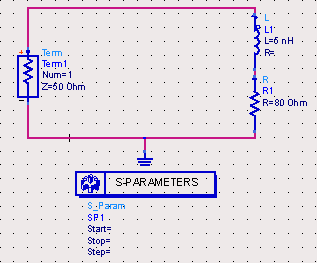
\includegraphics{I2_a_circuit.PNG}
   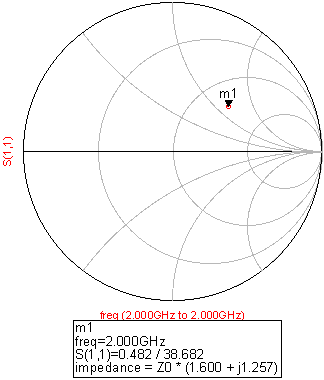
\includegraphics{I2_a_smith.PNG}

   Lorsque l’on ajoute une ligne de transmission entre la source et la charge, on obtient une impédance ramenée au niveau du port d’entrée de $z_E = \cfrac{z_L +j \tan{\beta d}}{1 + j z_L \tan{\beta d}}=\cfrac{z_L +j \tan{E}}{1 + j z_L \tan{E}}$

   Coefficient de réflexion correspondant : $\Gamma=\cfrac{z_E-1}{z_E+1}$

   Dans le cas particulier d’une ligne quart d’onde, ceci donne $-0.38-i0.30$

   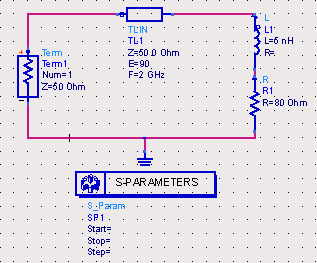
\includegraphics[width=8cm]{I2_b_circuit.PNG}
   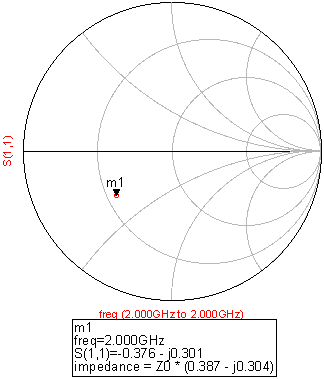
\includegraphics[width=8cm]{I2_b_smith.PNG}

   En utilisant l’outil «Tune», on peut modifier la longueur de la ligne en temps réel et voir le point se déplacer sur l’abaque de smith (ce qui peut être utile pour des réglages) :

   \includegraphics[width=8cm]{I2_c_0.jpg}
   \includegraphics[width=8cm]{I2_c_15.jpg}
   \includegraphics[width=8cm]{I2_c_30.jpg}
   \includegraphics[width=8cm]{I2_c_45.jpg}

   Cependant, on ne voit les points que un par un % TODO quel est le lieu des impédances blablabla

   On peut donc utiliser le «sweep parameter», qui permet sur la même abaque de voir tous les points :
   
   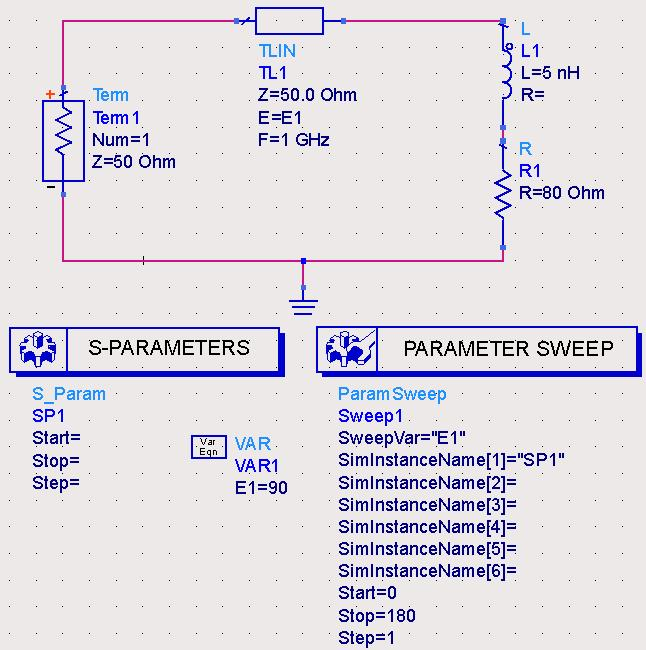
\includegraphics[width=8cm]{I2_d_circuit.jpg}
   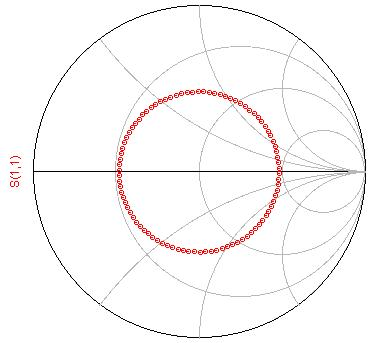
\includegraphics[width=8cm]{I2_d_simulation.jpg}

   Lorsque l’on enlève la bobine afin de ne garder que la partie réele de la charge, l’impédance ramenée dans le plan du port est donc la partie réele de celle que nous avions précédement : $z_L=\cfrac{Z_L}{Z_0}=\cfrac{80}{50} = 1.6$ ; ce que l’on vérifie sous ADS :

   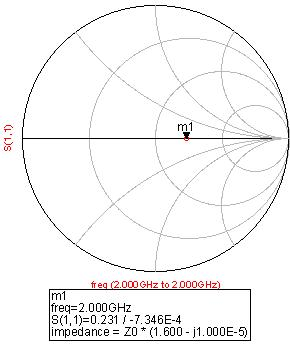
\includegraphics[width=8cm]{I2_e_impedance.jpg}

   On cherche maintenant à déterminer l’impédance de ligne $Z_C$ permettant d’obtenir une impédance ramenée $Z_E$ de 50 \Omega :
   $Z_E = Z_C \cfrac{Z_L +j Z_C\tan{\beta d}}{Z_C + j Z_L \tan{\beta d}} 
   \simeq Z_C \cfrac{j Z_C \tan{E}}{j Z_L \tan{E}}
   \simeq \cfrac{Z_C^2}{Z_U}$, 
   Donc pour $Z_E=50$, on a $Z_C=\sqrt{Z_E Z_L} = 63,25 \Omega$

   On vérifie la position du point sur ADS :

   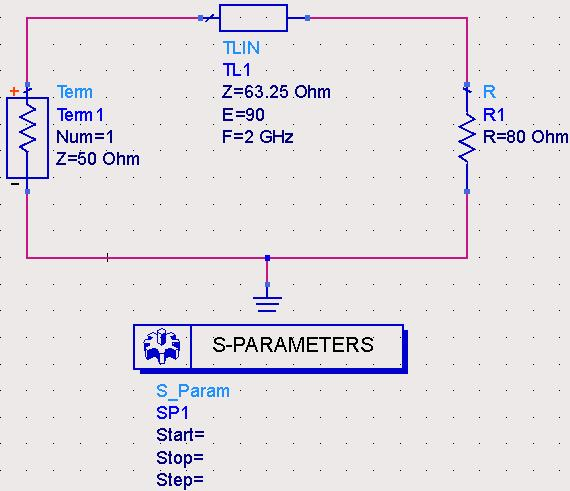
\includegraphics[width=8cm]{I2_e_50-circuit.jpg}
   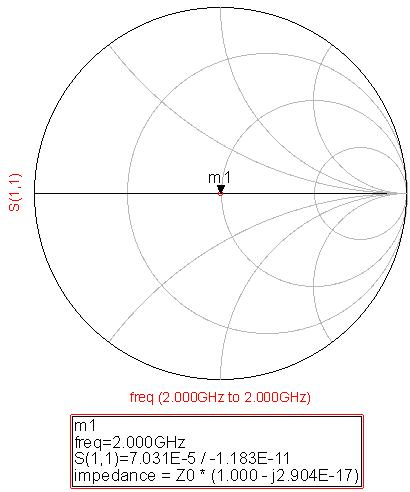
\includegraphics[width=8cm]{I2_e_50-simulation.jpg}

   On peut visualiser le lieu des charges ramenées en fonction des impédances de la ligne, avec un «sweep parameter» :

   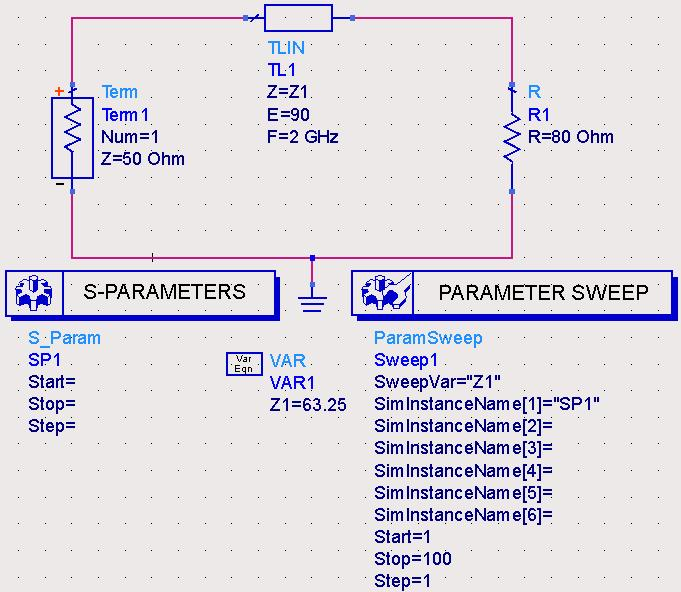
\includegraphics[width=8cm]{I2_e_impedances-circuit.jpg}
   \includegraphics[width=8cm]{I2_e_impedanceimpedances-simulation.jpg}



 \part{Annexes}
  Voici le fichier Scilab contenant tous les calculs :
  %\inputminted{scilab}{calculs.sci}



\end{document}
